\subsection{正部与负部}

定义4. --- 在格序群G中，元素 \(x \in G\) 的正部（相应地，负部，绝对值）是元素 \(\sup(x, 0)\) （相应地 \(\sup(-x, 0)\) , \(\sup(x, -x)\) ），记作 \(x^{+}\) （相应地 \(x^{-}\) , \(|x|\) ）。

\pandocbounded{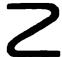
\includegraphics[keepaspectratio]{images/part002_7ee71349.jpg}}

尽管名称如此，负部 \(x^{-}\) 是一个正元素。

显然 \(x^{-} = (-x)^{+}\) 且 \(|-x| = |x|\) 。我们还注意到下列公式，其中第一个是定义以及序在平移下的不变性的直接推论，第二个则由第一个根据VI第10页命题7得出：

\[
\left\{ \begin{array}{l} \sup (x, y) = x + (y - x) ^ {+}, \\ \inf (x, y) = y - (y - x) ^ {+}. \end{array} \right.\tag{3}
\]

命题9. --- a) 对格序群G的每个元素 x，我们有 \(x = x^{+} - x^{-}\) 且 \(\inf(x^{+}, x^{-}) = 0\) 。

\begin{enumerate}
\def\labelenumi{\alph{enumi})}
\setcounter{enumi}{1}
\item
  对 \(x\) 作为两个正元素之差的每一种表示，设 \(x = u - v\) ，我们有 \(u = x^{+} + w\) 与 \(v = x^{-} + w\) ，其中 \(w = \inf(u, v)\) 。特别地，若 \(\inf(u, v) = 0\) ，则 \(u = x^{+}\) 且 \(v = x^{-}\) 。
\item
  关系 \(\ll x\leqslant y\gg\) 等价于 \(\ll x^{+}\leqslant y^{+}\) 且 \(x^{-}\geqslant y^{-}\gg\) 。
\item
  我们有 \(|x| = x^{+} + x^{-} \geqslant 0\) 。
\item
  对任意 \(x\) 与 \(y\) （在 \(G\) 中），我们有不等式 \(|x + y| \leqslant |x| + |y|\) ，并且更一般地 \(\left|\sum_{i=1}^{n} x_i\right| \leqslant \sum_{i=1}^{n} |x_i|\) （对元素的任意有限族 \((x_i)\) ，其元素属于 \(G\) ）。
\item
  对任意 \(x\) 与 \(y\) （在 \(G\) 中），我们有 \(||x| - |y|| \leqslant |x - y|\) 。
\end{enumerate}

我们将同时证明 \(a)\) 与 \(b)\) 。若 \(x = u - v\) ，其中 \(u\) 与 \(v\) 为正，则 \(u \geqslant x\) ，所以 \(u \geqslant \sup (x, 0) = x^{+}\) ，且 \(w = u - x^{+}\) 为正。另一方面，我们有

\[
x ^ {+} - x = \sup (x, 0) - x = \sup (x - x, - x) = x ^ {-}
\]

由此可得 \(x = x^{+} - x^{-}\) ，以及 \(v - x^{-} = w\) 。若 \(z \leqslant x^{-}\) ，则 \(z \leqslant x^{+} - x\) ，因此 \(x \leqslant x^{+} - z\) ；若还有 \(z \leqslant x^{+}\) ，则 \(x^{+} - z\) 是正的，因此 \(x^{+} \leqslant x^{+} - z\) （按 \(x^{+}\) 的定义）。于是我们有 \(z \leqslant 0\) ，这意味着 \(\inf(x^{+}, x^{-}) = 0\) ，从而通过平移得到 \(\inf(u, v) = w\) 。

\begin{enumerate}
\def\labelenumi{\alph{enumi})}
\setcounter{enumi}{2}
\item
  关系 \(x \leqslant y\) 蕴含 \(\sup (y, 0) \geqslant x\) 与 \(\sup (y, 0) \geqslant 0\) ，因此 \(x^{+} \leqslant y^{+}\) ；类似地，若 \(-y \leqslant -x\) ，我们推出 \(x^{-} \geqslant y^{-}\) 。相反的蕴含关系由 \(x = x^{+} - x^{-}\) 与 \(y = y^{+} - y^{-}\) 立即得出。
\item
  由于 \(x \leqslant x^{+}\) 且 \(-x \leqslant x^{-}\) ，显然
\end{enumerate}

\[
\left| x \right| = \sup (x, - x) \leqslant x ^ {+} + x ^ {-}.
\]

反之，若 \(a \geqslant x\) 且 \(a \geqslant -x\) ，则由 \(c\) ) 推出 \(a^+ \geqslant x^+\) , \(a^+ \geqslant x^-\) , \(a^- \leqslant x^-\) 与 \(a^- \leqslant x^+\) ；由于 \(a^-\) 是正的且 \(\inf(x^+, x^-) = 0\) ，后两个不等式推出 \(a^- = 0\) 且 \(a = a^+\) ；前两个不等式随后给出 \(a \geqslant \sup(x^+, x^-)\) ，而 \(\sup(x^+, x^-)\) 等于 \(x^+ + x^-\) （由 \(a\) ）以及VI第10页命题7）。

\begin{enumerate}
\def\labelenumi{\alph{enumi})}
\setcounter{enumi}{4}
\item
  由于 \(x \leqslant |x|\) 且 \(y \leqslant |y|\) ，我们有 \(x + y \leqslant |x| + |y|\) ；由于 \(-x \leqslant |x|\) 且 \(-y \leqslant |y|\) ，我们有 \(-x - y \leqslant |x| + |y|\) ；由此得到第一个不等式。第二个不等式通过对 \(n\) 作归纳得到。
\item
  把 \(x\) 与 \(y\) 分别换成 \(y\) 与 \(x - y\) （在 \(e\) ) 中），我们得到
\end{enumerate}

\[
\left| x \right| - \left| y \right| \leqslant \left| x - y \right|;
\]

类似地，我们有 \(|y| - |x| \leqslant |y - x| = |x - y|\) ；由此得出所述结果。

注记. --- 我们由 \(d\) 推出， \(|x|=0\) 蕴含 \(x=0\) （因为 \(x^{+}\) 与 \(x^{-}\) 都是正的）；于是 \(x\neq0\) 蕴含 \(|x|>0\) 。

命题9（DIV）. --- 若由 K 的主分式理想组成的群 \(\mathcal{P}^*\) 是格序的，则每个元素 \(x\) （属于 \(\mathbf{K}^*\) ）都可以写成 \(x = uv^{-1}\) 的形式，其中 \(u\) 与 \(v\) 是 A 的元素，满足 \(1 = \gcd(u, v)\) ；对任何其他表达式 \(x = u'v'^{-1}\) （它把 \(x\) 表示为 A 中两个元素之商） ，我们有 \(u' = uw\) 与 \(v' = vw\) ，其中 \(w\) 是 \(u'\) , \(v'\) 的一个最大公因子；特别地，若 \(1 = \gcd(u', v')\) ，则 \(u'\) 与 \(v'\) 分别是 \(u\) 与 \(v\) 的相伴元。

这样一个表达式 \(uv^{-1}\) （对 \(K^{*}\) 中一个元素 x 而言）通常称为既约分数。

